\documentclass[a4paper,12pt]{article}
\usepackage[spanish]{babel}
\hyphenation{co-rres-pon-dien-te}
%\usepackage[latin1]{inputenc}
\usepackage[utf8]{inputenc}
\usepackage[T1]{fontenc}
\usepackage{graphicx}
\usepackage[pdftex,colorlinks=true, pdfstartview=FitH, linkcolor=blue,
citecolor=blue, urlcolor=blue, pdfpagemode=UseOutlines, pdfauthor={H. Asorey},
pdftitle={Física 1A - Guía 05}]{hyperref}
\usepackage[adobe-utopia]{mathdesign}

\hoffset -1.23cm
\textwidth 16.5cm
\voffset -2.0cm
\textheight 26.0cm

%----------------------------------------------------------------
\begin{document}
\title{
{\normalsize{Universidad Nacional de Río Negro - Profesorados de Física y
Química}}\\ Física I A \\ Guía 06 - Cantidad de Movimiento}
\author{Asorey - Cutsaimanis}
\date{2016}
\maketitle

\begin{enumerate}
	\setcounter{enumi}{33}      %% Offset en numero de problema
	\item Calcule el vector cantidad de movimiento total $\vec p_T$ en cada uno
		de los siguientes casos:
		\begin{enumerate}
			\item un cuerpo de masa $m=2$\,kg que se mueve con velocidad $\vec
				v=5 \hat i$\,m\,s$^{-1}$,
			\item un automóvil de masa $m=1200$\,kg y velocidad $\vec u=100
				\hat i$\,km\,h$^{-1}$
			\item dos automóviles de masa $m_1=1000$\,kg y $m_2=1600$\,kg y
				velocidades $\vec u_1=20 \hat i$\,m\,s$^{-1}$ y $\vec u_2=40
				\hat i $\,m\,s$^{-1}$
			\item dos automóviles de masa $m_1=1000$\,kg y $m_2=1600$\,kg y
				velocidades $\vec u_1=40 \hat i$\,m\,s$^{-1}$ y $\vec u_2=-20
				\hat i$\,m\,s$^{-1}$
			\item dos automóviles de masa $m_1=1000$\,kg y $m_2=1600$\,kg y
				velocidades $\vec u_1=40 \hat i$\,m\,s$^{-1}$ y $\vec u_2=20
				\hat j$\,m\,s$^{-1}$
			\item un automóvil de masa $m=900$\,kg y velocidad
				$u=130$\,km\,h$^{-1}$ y un camión de masa $M=30000$\,kg y
				velocidad $u=80$\,km\,h$^{-1}$ con igual dirección pero
				sentidos opuestos
			\item Ocho esferas de igual masa $m=1$\,kg, que se mueven cada una
				con la misma rapidez $1$\,s$^{-1}$ y en sentido N, NE, E, SE,
				S, SO, O y NO respectivamente.
		\end{enumerate}
	\item Imagine dos cuerpos de masas $m_1$ y $m_2=3 m_1$ que se encuentran en
		reposo ($u_1=u_2=0$). Ambos cuerpos están unidos por un resorte de masa
		despreciable y cuya constante elástica vale $k=1000$\,N\,m$^{-1}$. El
		resorte está comprimido $\Delta x=0.5$\,m respecto de su posición de
		equilibrio. Una vez liberado el resorte, encuentre la relación entre
		las velocidades $\vec v_1$ y $\vec v_2$ de cada cuerpo. Luego calcule
		dichas velocidades y, suponiendo que $m_1=10$\,kg, calcule la energía
		cinética de cada cuerpo. Finalmente, compare la energía cinética del
		sistema con la potencial elástica inicial. ¿Qué conclusiones puede
		sacar?
	\item Un fuego artificial de masa $m=1$\,kg se encuentra en reposo en el
		instante en que estalla, separándose en $100$ partes de masa que
		podemos suponer iguales entre si, es decir $m_i=m/100$. Luego de la
		explosión, estos fragmentos se mueven en distintas direcciones y
		sentidos pero todos con la misma rapidez $v=1$\,m\,s$^{-1}$. Calcule el
		vector cantidad de movimiento total $\vec p_f$ luego de la explosión.
		Justifique.
    \vspace{-2.5cm}
	\item
		\begin{minipage}[t]{0.695\textwidth}
			Un péndulo balístico es un dispositivo utilizado para determinar el
			poder de fuego de un arma. Consiste en un péndulo formado por una
			bloque de madera de masa $M=5.98$\,kg que pende de un hilo de
			longitud $d=1.5$\,m (considerar que esa es la distancia entre el
			anclaje del péndulo y el centro del bloque). Una bala de masa
			$m=20$\,g es disparada por un revolver e impacta en el centro del
			bloque de madera. Tras el impacto, el bloque se eleva hasta formar
			un ángulo de $\theta=15^\mathrm{o}$ respecto a la vertical. ¿Cuál
			es la velocidad de la bala al salir del revolver?
		\end{minipage}
		\begin{minipage}[]{0.295\textwidth}
			\vspace{2.5cm}
			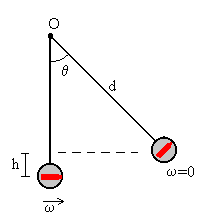
\includegraphics[width=0.7\textwidth]{balistico.png}
		\end{minipage}
	\item Dos astronautas de masas $m_1=70$\,kg y $m_2=80$\,kg, se encuentran
		originalmente en reposo entre si, trabajando fuera de la estación
		espacial. El astronauta de masa $m_1$ le pide a $m_2$ que le alcance un
		martillo, de masa $m_m=3$\,kg, quien se lo lanza con velocidad
		$v_m=2$\,m\,s$^{-1}$. El astronauta $m_1$ lo ataja sin dificultad.
		Calcule el vector velocidad final del astronauta 1 (con el martillo) y
		del astronauta 2.
	\item Un fiat uno de masa $m_1=600$\,kg se encuentra originalmente en
		reposo ($u_1=0$\,m/s) en el medio de la ruta por un problema mecánico.
		El conductor, que bajó a realizar una llamada telefónica al auxilio
		mecánico, nota que un camión de masa $m_2=30000$\,kg se desplaza hacia
		el fiat con velocidad $u_2=100$\,km/h. El desastre fue inevitable.
		Calcule la velocidad final $v$ del amasijo ($m_1+m_2$) resultante, y la
		variación de energía cinética del sistema.
	\item Repita los cálculos anteriores pero ahora suponga que el camión está
		detenido y el fiat uno es el que choca al camión. ¿Que puede decir de
		la transferencia de cantidad de movimiento en cada caso? ¿y con las
		pérdidas de energía cinética?  
	\item Un cuerpo de masa $m_1$ se desplaza con velocidad $u_1$ y experimenta
		una colisión totalmente inelástica con un cuerpo de masa $m_2$ que se
		mueve con velocidad $u_2$. Calcule la velocidad final del cuerpo
		resultante, de masa $m_1+m_2$, en cada uno de los siguientes casos: a)
		$m_1=m_2$ y $u_1=u_2$; b) $m_1=m_2$ y $u_1=-u_2$; c) $m_1=10 m_2$ y
		$u_1=u_2$; d) $m_1=10 m_2$ y $u_2=0$; e) $m_1=10 m_2$ y $u_1=10 u_2$.
	\item Una bola de billar de masa $m_1=0.2$\,kg se mueve con velocidad
		inicial $u_1=1$\,m/s y colisiona frontal y elásticamente con otra bola
		de billar de masa $m_2$ que se encuentra inicialmente en reposo
		($u_2=0$). Calcule la velocidad final de cada bola en los siguientes
		casos: a) $m_2=0.001 m_1$; b) $m_2=0.05 m_1$;  c) $m_2=0.9 m_1$; d)
		$m_2=m_1$; f) $m_2=1.1 m_1$; g) $m_2=20 m_1$; h) $m_2=1000 m_1$.
	\item En un reactor nuclear los neutrones ($m_1=1$\,uma\footnote{La uma
		(unidad de masa atómica) es una unidad de masa ampliamente utilizada en
		química, bioquímica (usualmente se la llama Dalton), y en física
		nuclear, y que equivale a la masa de doceava parte del átomo de
		$^{12}$C, 1\,uma$\simeq 1.67 \times 10^{-27}$\,kg}), chocan frontal y
		elásticamente con moléculas de agua pesada ($D_2O$, $m_2=20$\,uma) en
		un proceso denominado moderación. Suponiendo que la velocidad del
		neutrón es $u_1=1000$\,m\,s$^{-1}$ y las moléculas de agua pesada están
		inicialmente en reposo ($u_2=0$), calcule:
		\begin{enumerate}
			\item Las velocidades de la molécula de agua y del neutrón luego de
				la primer colisión, y la variación de energía cinética para el
				neutrón y la molécula de agua pesada
			\item El número de colisiones necesarias para que la velocidad del
				neutrón se reduzca al $0.1\%$ de $u_1$.
		\end{enumerate}
\end{enumerate}
\end{document}
%%%%
